\section{Постановка задачи}
Чип быстрой аналоговой памяти PSI DRS4 имеет 8 каналов, каждый из которых содержит 1024 ячейки. Они включают конденсаторы для хранения значения заряда и электронные ключи для записи сигналов и считывания напряжений через АЦП (аналого-цифровой преобразователь). Ячейки объединяются в кольцевые буферы. При подаче сигнала синхронизации запись напряжений на конденсаторы прекращается, а номер ячейки (в которую была сделана последняя запись) запоминается.

\begin{figure}[H]
    \centering
    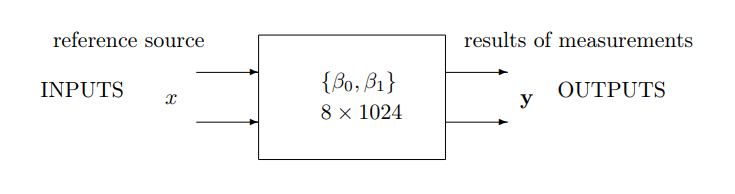
\includegraphics[width=1\linewidth]{image/Chip.png}
    \caption{Структурная схема калибровки DRS4}
    \label{fig:chip}
\end{figure}

Ставится задача калибровки данного чипа. Для этого на входы платы подается набор напряжений постоянного значения, охватывающий рабочий диапазон микросхемы. Для каждого отдельного напряжения $X$, эта операция повторяется 100 раз. На основе полученных данных для каждой ячейки рассчитываются линейные регрессии. 

Таким образом, калибровка сводится к определению параметров линейной регрессии 

\begin{equation}
    Y = \beta_0 X + \beta_1.
\end{equation}